\documentclass[12pt]{article}

\usepackage[a4paper,left=25mm,right=25mm,top=35mm,bottom=25mm]{geometry}
\usepackage{ngerman}
\usepackage{parskip}
\usepackage{times}
\usepackage{graphicx}
\usepackage{listings}
\usepackage{fancyhdr}
\usepackage{float}
\usepackage{amsmath}

\setlength{\headheight}{15.2pt}
\pagestyle{fancy}

\lhead{Bildverarbeitung und Mustererkennung\\Praktikum Blatt 6}
\rhead{Patrick Hüntelmann\\27.05.2022}

\lstset{
  basicstyle=\ttfamily,
  breakatwhitespace=false,         % sets if automatic breaks should only happen at whitespace
  breaklines=true,                 % sets automatic line breaking
  captionpos=b,                    % sets the caption-position to bottom
  deletekeywords={...},            % if you want to delete keywords from the given language
  escapeinside={\%*}{*)},          % if you want to add LaTeX within your code
  extendedchars=true,              % lets you use non-ASCII characters; for 8-bits encodings only, does not work with UTF-8
  frame=single,	                   % adds a frame around the code
  keepspaces=true,                 % keeps spaces in text, useful for keeping indentation of code (possibly needs columns=flexible)
  language=python,                 % the language of the code
  showstringspaces=false,          % underline spaces within strings only
  showtabs=false,                  % show tabs within strings adding particular underscores
  tabsize=2,	                   % sets default tabsize to 2 spaces
}

\begin{document}

\pagenumbering{arabic}

\section*{Aufgabe 6}
\subsection*{Teil 1. Morphologische Operatoren}
Die morphologische Operation \textit{opening} ist in der Funktion \textbf{aufgabe\_1} (main.py Zeile 84) implementiert.
Diese Funktion lädt das Bild, baut eine Kernel-Struktur auf und initialisiert die Anzahl der Iterationen. Anschließend führt diese für die Anzahl der Iterationen $n$, $n$-mal eine Dilatation des Bildes und anschließend $n$-mal eine Erosion des Bildes mit der zuvor aufgebauten Struktur durch.
Die Dilatation ist in der Funktion \textbf{dilate} (main.py Zeile 17) und die Erosion in der Funktion \textbf{erode} (main.py Zeile 49) implementiert.

\subsubsection*{Ergebnisbilder}
\begin{figure}[H]
  \centering
  
\includegraphics[width=0.4\textwidth, keepaspectratio]{dilated.png}\\
  Dilatation 5x5 Struktur, 2 Iterationen
\end{figure}
\begin{figure}[H]
  \centering
  
\includegraphics[width=0.4\textwidth, keepaspectratio]{eroded.png}\\
  Erosion 5x5 Struktur, 2 Iterationen
\end{figure}

\newpage

\subsection*{Teil 2. Segmentierung}
Die Verwendung des \textit{Wasserscheidentransformation} mit dazugehöriger Vorverarbeitung ist in der Funktion \textbf{aufgabe\_2} (main.py Zeile 116) implementiert.
Diese Funktion extrahiert den Blaukanal des Bildes und führt auf diesem zunächst ein Thresholding mit dem Otsu-Verfahren, anschließend eine \textit{opening}-Morphologische Transformation durch.
Anschließend wird mit einer weiter Dilatation die Hintergrund-Informationen aus dem Bild extrahiert und eine Distanz-Transformation durchgeführt und mit dieser die Vordergrund-Informationen extrahiert. Mit einer Subtraktion des Vordergrundes vom Hintergrund wird der Unbekannte Zwischenbereich bestimmt und anhand dessen Marker auf dem Bild erstellt. Mit diesen Markern wird dann die \textit{Wasserscheidentransformation} durchgeführt mit welcher auf dem Ergebnisbild die unterschiedlichen Segmente umrandet und mit Labels gekennzeichnet werden.

\subsubsection*{Ergebnisbilder}
\begin{figure}[H]
  \centering
  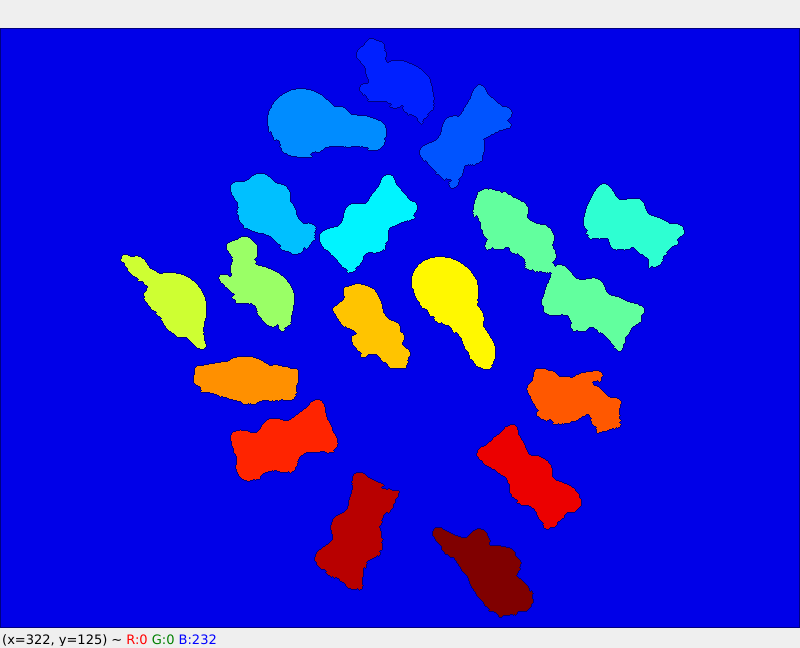
\includegraphics[width=0.55\textwidth, keepaspectratio]{marker.png}\\
  Marker-Bild (JET-Colormap)
\end{figure}
\begin{figure}[H]
  \centering
  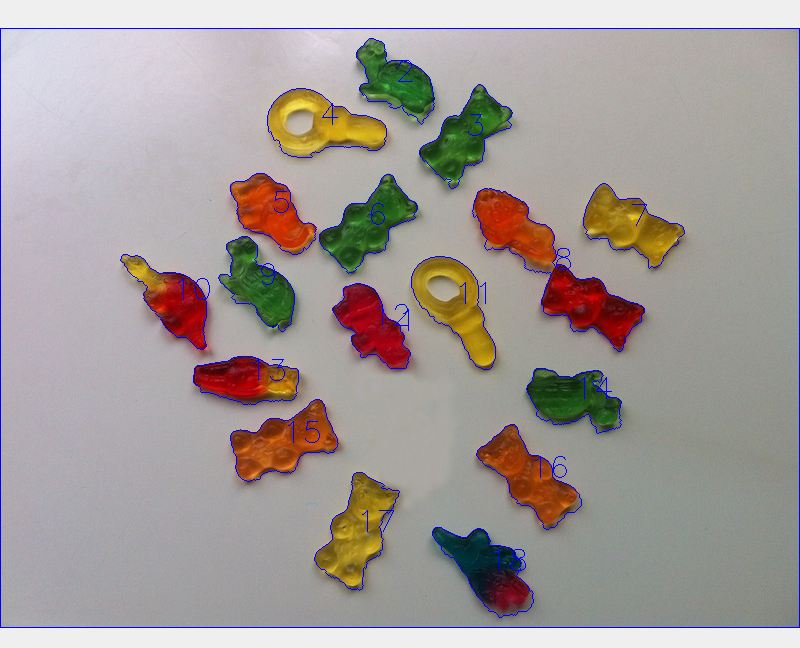
\includegraphics[width=0.55\textwidth, keepaspectratio]{outline.png}\\
  Ergebnisbild mit Umrandung der Regionen und Labels
\end{figure}

\end{document}
